
\lecture{Hypothesis Testing}{hypothesis-testing}
\section{Hypothesis Testing}

\title{Hypothesis Testing Where the Standard Deviation is Known}
\subtitle{Is there a difference?}

%\author{Kelly Black}
%\institute{Clarkson University}
\date{29 March 2013}

\begin{frame}
  \titlepage
\end{frame}

\begin{frame}
  \frametitle{Outline}
  \tableofcontents[hideothersubsections,sectionstyle=show/hide]
\end{frame}



\subsection{Clicker Quiz}



\begin{frame}
  \frametitle{Clicker Quiz}

  % \begin{clickerQuiz}

  \iftoggle{clicker}{%
    
    Cereal is produced at one of your factories. You are told that the
    mean contents is 417.3g per box. You suspect that this is too
    high. 

    What hypothesis test would you form to test this? \\
    ~ \\
    \begin{tabular}{ll@{\hspace{3em}}l}
      A & $H_0$: The mean is less that 417.3g  \\
        & $H_a$: The mean is  417.3g \\
      ~ \\
      B & $H_0$: The mean is 417.3g \\
        & $H_a$: The mean is more than 417.3g \\
      ~ \\
      C & $H_0$: The mean is 417.3kg  \\
        & $H_a$: The mean is less than 417.3kg 
    \end{tabular}

  }

  %\end{clickerQuiz}
  

\end{frame}


\subsection{Hypothesis Testing}

\begin{frame}{Hypothesis Testing: The Idea}

  You do not ``prove'' your hypothesis. Instead you gather
  (circumstantial) evidence against a counter-situation.

  \begin{itemize}
  \item You have a hypothesis, call it the alternate hypothesis.
  \item You have null hypothesis ($H_0$) that \textit{\color{red}you think is not correct}.
  \item Assume that $H_0$ is correct.
  \item Gather the evidence (for us: data)
  \item Decide if your result is \textit{\color{red}unlikely \underline{given}
      your assumptions}.
  \end{itemize}

  \only<2->%
  {

    There are two ways to do this. The first is the \textit{Classical
      Approach}, and the second is the the $p$-value approach. You
    need to know how both approaches work because different people
    have different preferences, and you have to know how to react.

  }

\end{frame}

\begin{frame}
  \frametitle{Left Sided Test of the Mean}

  You think that the mean is lower.

  \begin{columns}
    \column{0.25\textwidth}
    \begin{eqnarray*}
      \begin{array}{lrcl}
        H_0: & \mu & = & \# \\
        H_a: & \mu & < & \#
      \end{array}
    \end{eqnarray*}

    \column{0.75\textwidth}

    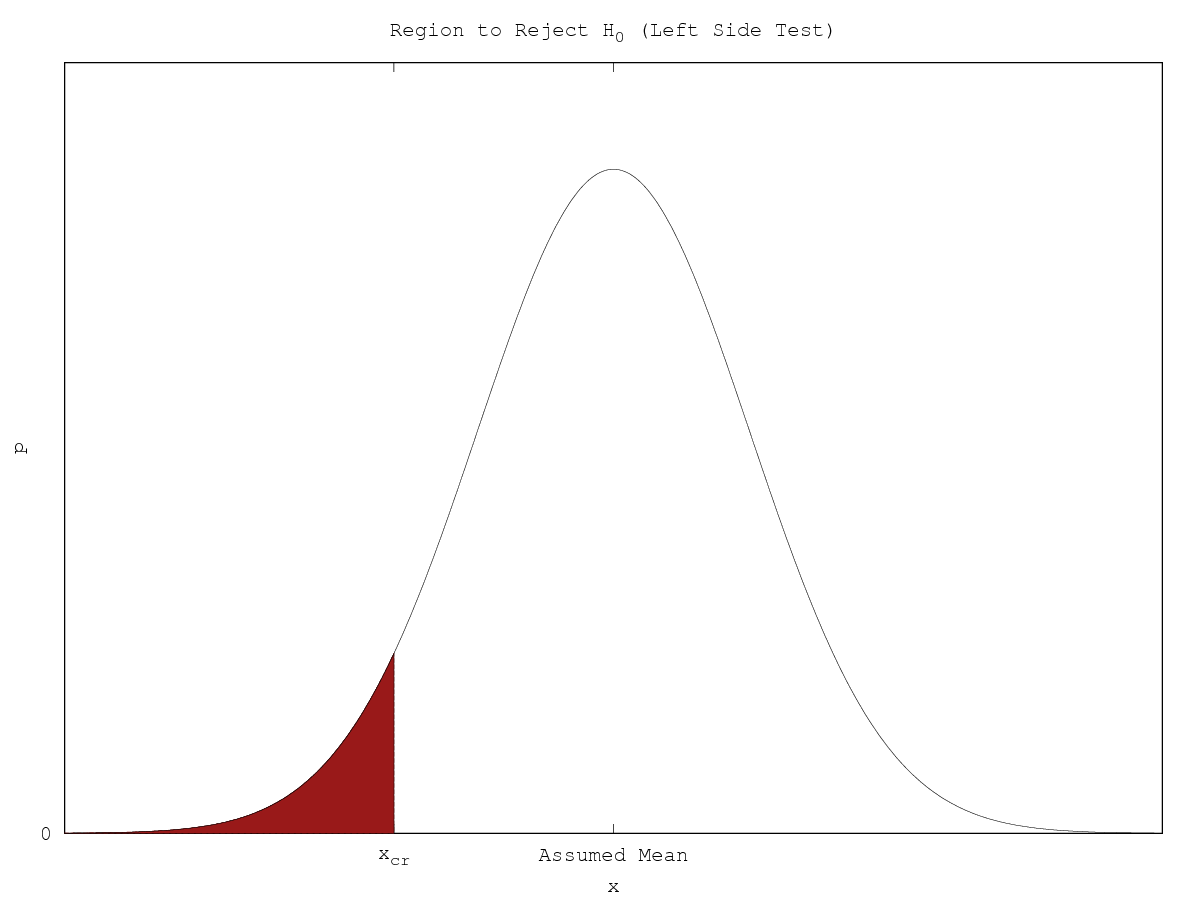
\includegraphics[width=5cm]{img/leftSideHypothesisTest}

  \end{columns}

  \begin{description}
  \item[$p$-value Approach] The probability that you do worse than
    $\bar{x}$ is the area to the left under the curve. If the area is
    smaller than the significance level ($\alpha$) then it is an
    \textit{unlikely result}.
  \item[Classical Approach] The area to the left of $x_{cr}$ is
    equal to the significance level ($\alpha$). If your $\bar{x}$ is
    less than this critical value then it is an \textit{unlikely
      result}.
  \end{description}


\end{frame}

\begin{frame}
  \frametitle{Right Sided Test of the Mean}

  You think that the mean is higher.

  \begin{columns}
    \column{0.25\textwidth}
    \begin{eqnarray*}
      \begin{array}{lrcl}
        H_0: & \mu & = & \# \\
        H_a: & \mu & > & \#
      \end{array}
    \end{eqnarray*}

    \column{0.75\textwidth}

    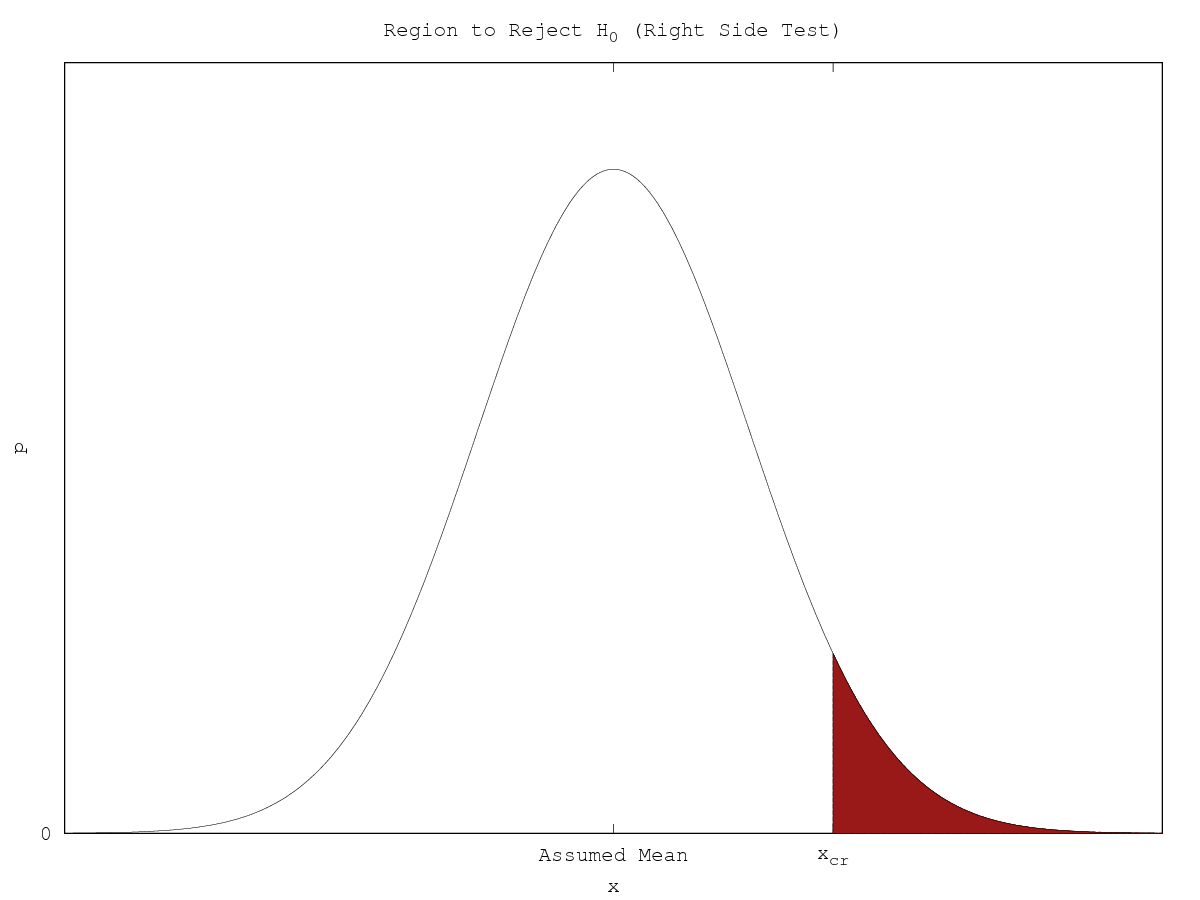
\includegraphics[width=5cm]{img/rightSideHypothesisTest}

  \end{columns}

  \begin{description}
  \item[$p$-value Approach] The probability that you do worse than
    $\bar{x}$ is the area to the right under the curve. If the area is
    smaller than the significance level ($\alpha$) then it is an
    \textit{unlikely result}.
  \item[Classical Approach] The area to the right of $x_{cr}$ is
    equal to the significance level ($\alpha$). If your $\bar{x}$ is
    more than this critical value then it is an \textit{unlikely
      result}.
  \end{description}


\end{frame}


\begin{frame}
  \frametitle{Two Sided Test of the Mean}

  \vspace*{-1em}

  You think that the mean is different.

  \begin{columns}
    \column{0.25\textwidth}
    \begin{eqnarray*}
      \begin{array}{lrcl}
        H_0: & \mu & = & \# \\
        H_a: & \mu & \neq & \#
      \end{array}
    \end{eqnarray*}

    \column{0.75\textwidth}

    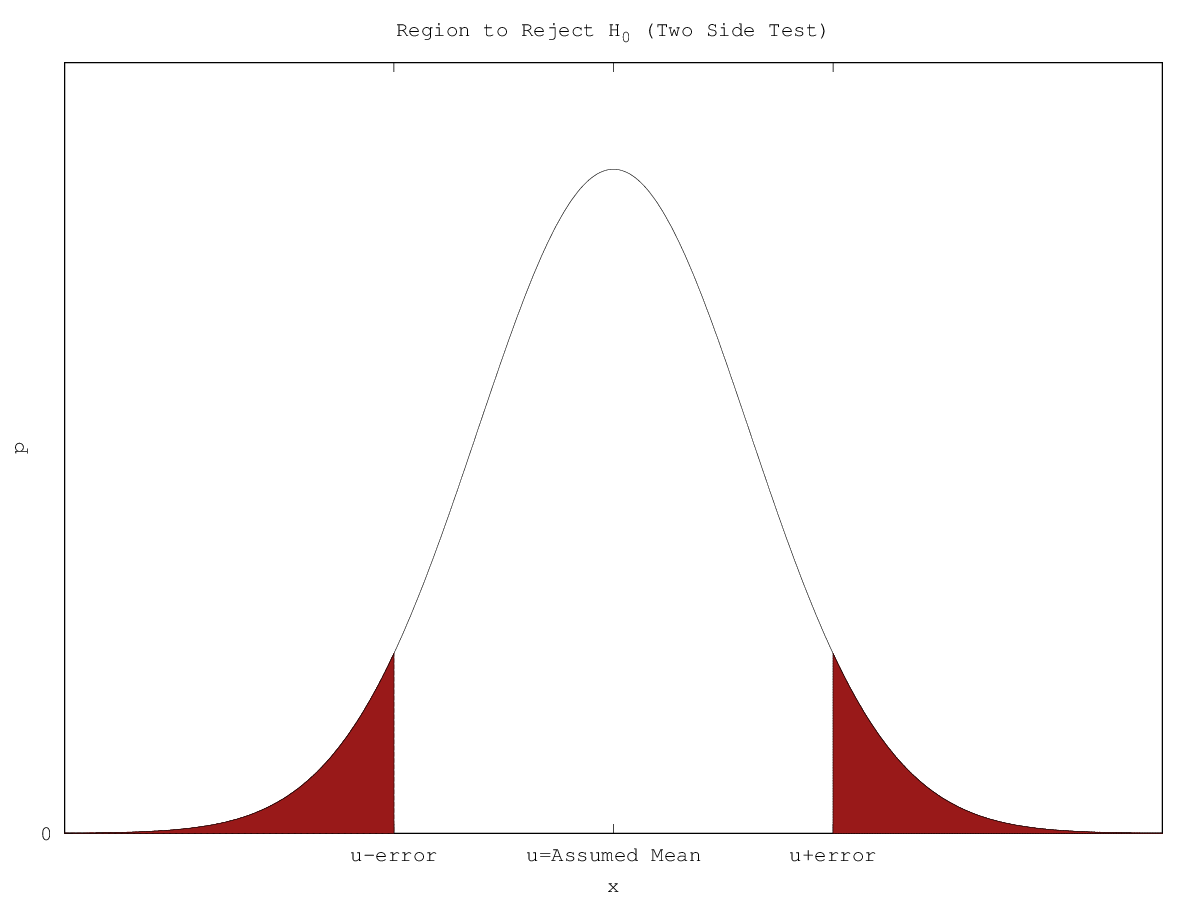
\includegraphics[width=5cm]{img/twoSideHypothesisTest}

  \end{columns}

  \begin{description}
  \item[$p$-value Approach] The probability that you do worse than
    $\bar{x}$ is the area to the left \textit{and} right under the
    curve. If the area is smaller than the significance level
    ($\alpha$) then it is an \textit{unlikely result}.
  \item[Classical Approach] The area to the left of
    $\mu-\mathrm{error}$ and to the right of $\mu+\mathrm{error}$ is
    equal to the significance level ($\alpha$). If your $\bar{x}$ is
    less than $\mu-\mathrm{error}$ or more than $\mu+\mathrm{error}$
    this critical value then it is an \textit{unlikely result}.
  \end{description}


\end{frame}



\subsection{Examples}

\subsection{Cereal Box Contents}

\begin{frame}{Cereal}

  Cereal is produced at one of your factories. You are told that the
  mean contents is 417.3g per box. You suspect that this is too
  high. 

  \vfill

  \only<2->
  {
    \begin{tabular}{l@{\hspace{2em}}l}
      $H_0$: & The mean is 417.3g \\
      $H_a$: & The mean is less than 417.3g 
    \end{tabular}
    \\ Use a 5\% significance level.
  }

  \vfill

  \only<3->
  {

    Sample fifteen boxes chosen at random, and ask if there is
    sufficient evidence to reject $H_0$. Suppose we find a sample mean
    of 412.4g and a {\color{red}standard deviation} of 12.0g.

  }

  \vfill

\end{frame}

\begin{frame}{Result}

  We \textbf{do not} have sufficient evidence to reject $H_0$ at the
  5\% significance level using a {\color{red}normal distribution} with fifteen
  samples and a {\color{red}standard deviation} of 12.0g.
  
\end{frame}



\subsection{Stock Price Change}

\iftoggle{clicker}{%
  \begin{frame}
    \frametitle{Clicker Quiz}

    We read that the mean change in the price of the stocks in a given
    sector changed by -0.55\$ with a standard deviation of 0.74\$. We
    suspect that the mean change is not that low.

    What hypothesis test would you form to test this? \\
    ~ \\
    \begin{tabular}{ll@{\hspace{3em}}l}
      A & $H_0$: The mean change is -0.55\$. \\
        & $H_a$: The mean change is more than -0.55. \\
      ~ \\
      B & $H_0$: The mean change is -0.55\$. \\
        & $H_a$: The mean change is less than -0.55\$. \\
        ~ \\
      C & $H_0$: The mean change is less than -0.55\$.  \\
        & $H_a$: The mean change is -0.55\$. \\
        ~ \\
      D & $H_0$: The mean change is more than -0.55\$.  \\
        & $H_a$: The mean change is -0.55\$.

      \end{tabular}

    \end{frame}
}


\begin{frame}{Stock Price}

  We read that the mean change in the price of the stocks in a given
  sector changed by -0.55\$ with a {\color{red}standard deviation} of 0.74\$. We
  suspect that the mean change is not that low.

  \vfill

  \only<2->
  {
    \begin{tabular}{l@{\hspace{2em}}l}
      $H_0$: & The mean change is -0.55\$. \\
      $H_a$: & The mean change is more than -0.55. 
    \end{tabular}
    \\ Use a 5\% significance level.
  }

  \vfill

  \only<3->
  {

    Sample one-hundred stocks chosen at random, and ask if there is
    sufficient evidence to reject $H_0$. Suppose that we find a sample
    mean of -0.42\$.

  }

  \vfill

\end{frame}

\begin{frame}{Result}

  We have sufficient evidence to reject $H_0$ at the 5\% significance
  level using a normal distribution with a one-hundred samples and a
  {\color{red}standard deviation} of 0.74\$.
  
\end{frame}


\subsection{Units Shipped}

\iftoggle{clicker}{%
  \begin{frame}
    \frametitle{Clicker Quiz}

    You are told that the mean number of units shipped per day at a
    particular factory is 135,000 units per day. You think that number
    is not correct.

    What hypothesis test would you form to test this? \\
    ~ \\
    \begin{tabular}{ll@{\hspace{3em}}l}
      A & $H_0$: The mean number of units is more than 135,000 units per day. \\
        & $H_a$: The mean number of units is 135,000 units per day. \\
        ~ \\
      B & $H_0$: The mean number of units is 135,000 units per day. \\
        & $H_a$: The mean number of units is more than 135,000 units per day. \\
        ~ \\
      C & $H_0$: The mean number of units is 135,000 units per day.  \\
        & $H_a$: The mean number of units is not 135,000 units per day. \\
        ~ \\
      D & $H_0$: The mean number of units is not 135,000 units per day.  \\
        & $H_a$: The mean number of units is 135,000 units per day.

      \end{tabular}

    \end{frame}
}


\begin{frame}{Units Shipped}


  You are told that the mean number of units shipped per day at a
  particular factory is 135,000 units per day. You think that number
  is not correct.

  \vfill

  \only<2->
  {
    \begin{tabular}{l@{\hspace{2em}}l}
      $H_0$: & The mean number of units is 135,000 units per day. \\
      $H_a$: & The mean number of units is not 135,000 units per day.
    \end{tabular}
    \\ Use a 5\% significance level.
  }

  \vfill

  \only<3->
  {

    Sample the daily output for twenty-five days chosen at random, and
    ask if there is sufficient evidence to reject $H_0$. Suppose we
    find a sample mean of 140,266 units per day and a standard
    deviation of 14,000 units per day.

  }

  \vfill

\end{frame}

\begin{frame}{Result}

  We \textbf{do not} have sufficient evidence to reject $H_0$ at the
  5\% significance level using a normal distribution with twenty-five
  samples and a {\color{red}standard deviation} of 14,000 units per day.
  
\end{frame}



% LocalWords:  Clarkson pausesection hideallsubsections hideothersubsections
% LocalWords:  sectionstyle
